\chapter{Theory}
\section{What is a resonator?}
By resonator we mean a harmonic oscillator within which some quantity varies harmonically with time. In case of a helical resonator an alternating current in electrical circuit periodically transfers the inductive energy stored in a magnetic field of the helix into the capacitive electric field energy between the helix and the shield. When being stimulated by an RF signal with a natural frequency of the system, voltage amplitude grows until the damping mechanisms are strong enough to balance the resonant effect.

\section{Helical resonator models}
In order to create a helical resonator satisfying our experimental conditions and limitations we inevitably come to a need for a theoretical model that would be able to predict the essential characteristics of the resulting unit. The following sections aim to provide an overview and comparison between the models.

\subsection{Macalpine \& Schildknecht}
\begin{figure}[h!]
	\centering
	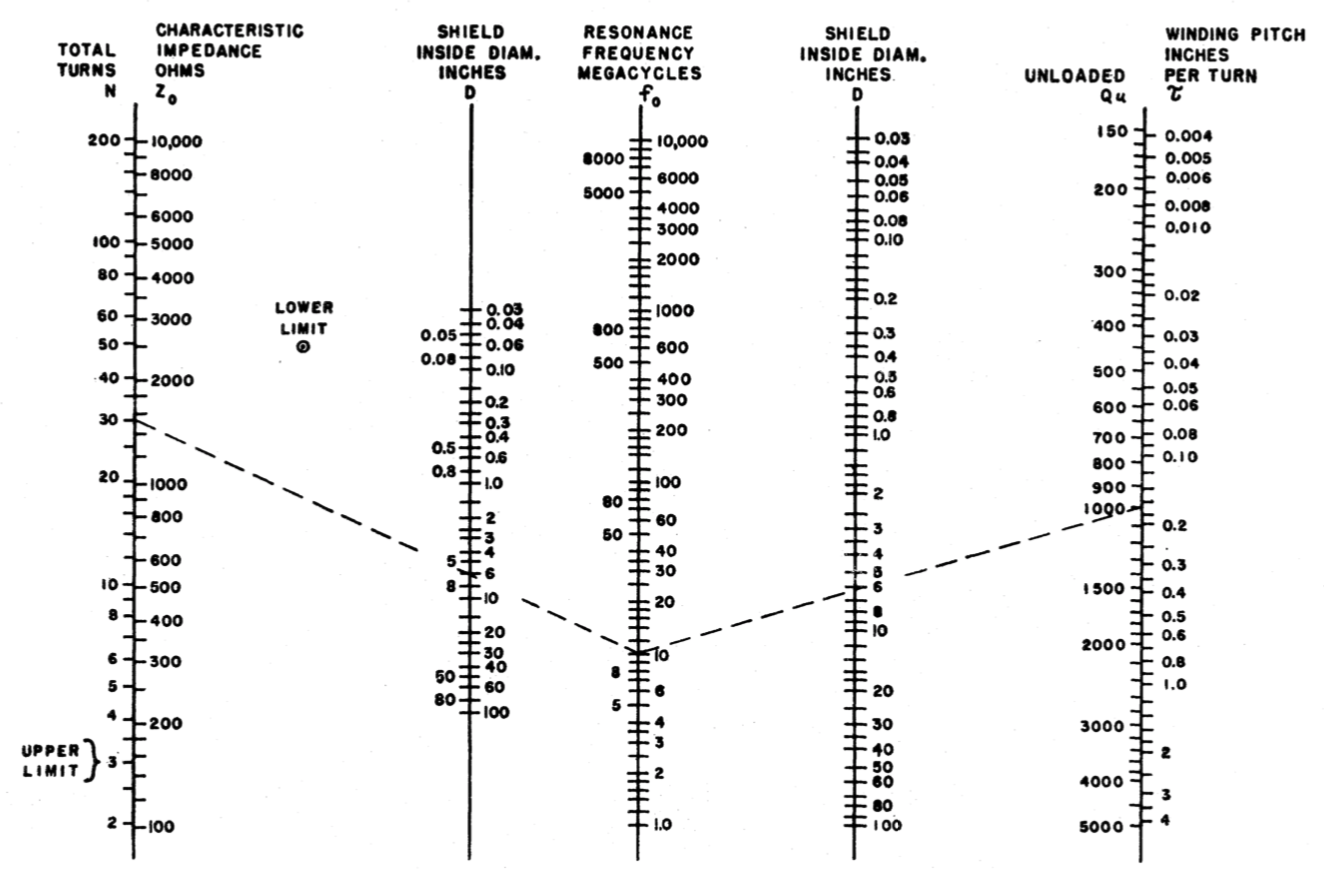
\includegraphics[width=.99\textwidth]{images/macalpine_chart}
	\caption{Design chart for quarter-wave helical resonators \cite{Macalpine2000}}
	\label{fig:macalpine_chart}
\end{figure}

A well-known approach \cite{Macalpine2000} for describing helical resonators was introduced in the same year as Richard Feynman's idea \cite{Feynman1960} to use quantum systems for computations. It was motivated by the possibility to reduce volume compared to TEM-mode coaxial-line resonators (90\% volume reduction for the reference case \cite{Macalpine2000}). While skipping a detailed theoretical analysis it nevertheless provides a basis for constructing a resonator: such as regions of usefulness, design considerations and a set of parameters' dependencies maximizing $Q$.

While describing essential properties of an unloaded helical quarter-wave resonator, this paper \cite{Macalpine2000} also predicts the shift of resonant frequency if an external load is connected. In order to define a new frequency one can make use of telegraph equations \cite{Rohde2009} by effectively treating the ion trap as a capacitor.

Important results of \cite{Macalpine2000} can be found in equations \ref{eq:macalpine} with parameters named as in the figure \ref{fig:helical_example}.
\begin{equation}
\begin{aligned}
	d/D &= 0.55\\
	b/d &= 1.5\\
	h &\approx (b + D/2)
\end{aligned}
\label{eq:macalpine}
\end{equation}
\subsection{Siverns et al.}
Unfortunately modeling an ion trap as a pure capacitive load is not always accurate. Introducing resistive losses imposes an additional shift of resonant frequency which pushes the deviation from self-resonant frequency even further. It is possible to tune the strength of the inductive coupling between the antenna and the main coil to compensate this shift while losing in efficiency.

These limitations of Macalpine's \& Schildknecht's \cite{Macalpine2000} model have been overcome in a newer paper \cite{Siverns2012} which takes the development of an amplifier, specifically for the needs of quantum computing, one step further. By taking a look at the joint resonator + ion trap system as a whole it aims to predict the effective $Q$ and frequency. This model ensures that it's possible to find optimal parameters for given experimental constraints.

While it is heavily recommended to check the original \cite{Siverns2012} paper to understand the theory behind calculations in appendix \ref{chapter:siverns_code} we will provide a short explanation of the exact usage below. All symbols correspond to \cite{Siverns2012}.

In our approach the only varying parameters are the diameter of a shield $D$ and the diameter of a helix $d$ with $\alpha = d / D$.

We take $d_0$ from Macalpine's calculations (see appendix \ref{chapter:macalpine_code}).
\begin{equation}
	d_0 = \text{Macalpine's}
\end{equation}
\begin{equation}
	\tau = 2*d_0
\end{equation}
Height of the coil is dependent on $D$ and size constrains. With this approach it might be less than zero, so this case needs to be handled.
\begin{equation}
	b = 56 \text{ mm} - D/2
\end{equation}
Number of turns in the coil $N$ can be derived from $b$ and $\tau$.
\begin{equation}
	N = b/\tau
\end{equation}
Calculating the coil self capacitance.
\begin{equation}
	C_C = \left( \left( 11.26 \frac{b}{d} \right) + 8 + \left( \frac{27}{\sqrt{b/d}} \right) \right) d \text{ pF}
\end{equation}
Calculating coefficients.
\begin{equation}
	K_{L_c} = 39.37 \; \frac{0.025 \; d^2 \left(1 - \alpha^2 \right)}{\tau^2} \; 10^{-6} \text{ H/m}
\end{equation}
\begin{equation}
	K_{C_s} = 39.37 \; \frac{0.75}{\log_{10}{(D/d)}} \text{ pF/m}
\end{equation}
Calculating the shield-coil capacitance.
\begin{equation}
	C_s = b* K_{C_c}
\end{equation}
Calculating the inductance of the coil.
\begin{equation}
	L_C = b* K_{L_c}
\end{equation}
Calculating the resonant frequency $\omega_{res}$. We only use it to determine whether it is close to the target frequency $\omega_0$ which would be actually used further in the calculations.
\begin{equation}
	\omega_{res} = \left( \left( C_s + C_t + C_w + C_c \right) L_C \right)^{-1/2}
\end{equation}
\begin{equation}
	\omega_0 = 2\pi * 40 \text{ MHz}
\end{equation}
Calculating the skin depth.
\begin{equation}
	\delta = \sqrt{\frac{2 \rho}{\omega_0 \; \mu_0}}
\end{equation}
Calculating the unwound length of the coil.
\begin{equation}
	l_c = 2\pi \; \sqrt{\left( \frac{d}{2} \right)^2 + \left( \frac{\tau}{2\pi} \right)^2} \; \frac{b}{\tau}
\end{equation}
Calculating the difference between the coil's and shield's radii.
\begin{equation}
	r = \frac{d}{2} \left( \alpha^{-1} - 1 \right)
\end{equation}
Calculating the number of ''turns`` in the currents path in the shield.
\begin{equation}
	N_s = \frac{b \; l_c}{4\pi \; r^2}
\end{equation}
Calculating the distance of the currents path in the shield.
\begin{equation}
	l_s = N_s \sqrt{\left( \frac{\pi \; d}{\alpha} \right)^2 + \left( \frac{b}{N_s} \right)^2}
\end{equation}
Calculating the resistance of a currents path in the shield.
\begin{equation}
	R_s = \frac{\rho \; l_s}{b \; \delta}
\end{equation}
Calculating the resistance of the coil.
\begin{equation}
	R_c = \frac{\rho \; l_c}{d_0 \; \pi \; \delta}
\end{equation}
Calculating the resistance of the solder joint dependent on a frequency with $3*10^{-3}$ Ohm being a typical resistance value for a DC current, which nevertheless ideally should be measured.
\begin{equation}
	R_j = 0.003 \; \sqrt{ \frac{\omega_0}{2\pi \; 10^5	} } \text{ Ohm}
\end{equation}
Calculating various reactances.
\begin{equation}
	X_{L_c} = \omega_0 \; L_C
\end{equation}
\begin{equation}
	X_{C_c} = \left( \omega_0 \; C_c \right)^{-1}
\end{equation}
\begin{equation}
	X_{C_t} = \left( \omega_0 \; C_t \right)^{-1}
\end{equation}
\begin{equation}
	X_{C_w} = \left( \omega_0 \; C_w \right)^{-1}
\end{equation}
\begin{equation}
	X_{C_s} = \left( \omega_0 \; C_s \right)^{-1}
\end{equation}
Calculating the impedance of the coil.
\begin{equation}
	Z_{coil} = \left( \left( \iu X_{L_c} + R_c \right)^{-1} + \left( X_{C_c} / \iu \right)^{-1} \right)^{-1}
\end{equation}
Calculating the equivalent impedance.
\begin{equation}
	Z_E = \left(  \left( X_{C_t}/\iu + R_t \right)^{-1} + \left( X_{C_w}/\iu \right)^{-1} + \left( X_{C_s}/\iu \right)^{-1} \right)^{-1}
\end{equation}
Calculating the total impedance.
\begin{equation}
	Z_{tot} = Z_{coil} + Z_E + R_s + R_j
\end{equation}
Calculating the real part of the total impedance.
\begin{multline}
	Z_{real} = \frac{R_c \; X^2_{C_c}}{R^2_c + \left( X_{C_c} - X_{L_c} \right)^2}\\ 
	+ \frac{R_t \; X_{C_s} \, X_{C_w}}{R^2_t \left( X_{C_s} + X_{C_w} \right)^2 + \left( X_{C_s} \left( X_{C_t} + X_{C_w} \right) + X_{C_t} \, X_{C_w} \right)^2}\\
	+ R_s + R_j
\end{multline}
Finally calculating the $Q$.
\begin{equation}
	Q = \frac{L_C \; \omega_0}{Z_{real}}
\end{equation}








\section{Comparison}
Macalpine's and Schildknecht's \cite{Macalpine2000} model gives insides for designing a helical quarter-wave resonator with a given self-resonant frequency. However major shifts from it can be expected when connecting the ion trap. Siverns' et al. approach \cite{Siverns2012} investigates connections between various parameters in the total circuit. As a result one could create a resonator which implements a transfer function closer to a desired one. Considering these benefits the Siverns model \cite{Siverns2012} was selected.